% Load the documentclass. thesis.sty was tested with book and scrbook
\documentclass[book]{scrbook}
% Load some useful packages for this document
\usepackage[demo]{graphicx}
\usepackage[final]{microtype}
\usepackage[utf8]{inputenx}
\usepackage{lmodern,mathpazo}
\linespread{1.05}
\usepackage[english]{babel}
\usepackage{colortbl,booktabs,blindtext}
\newcommand\thesis{\texttt{thesis.sty}}

% Load thesis.sty
\usepackage[consistency,styledtoc]{thesis}
\chapterboxheight=15ex
\chapterboxwidth=10em
\usetikzlibrary{patterns,intersections,snakes}

\title{Sample usage of the \thesis\ layout}
\author{Henri Menke {\rmfamily\itshape\&} Nicolai Lang}% don't use \and
\university{\textls{University of Stuttgart}}
\city{Anywhere}
\institute{Institute for Theoretical Physics}
\supervisor[Package written by]{Henri Menke}
\thesisname{Manual}% optional
\secondarycorrector[Based on a layout by]{Nicolai Lang}% optional
%\date{Yesterday}% optional
\thesisimage{% optional
  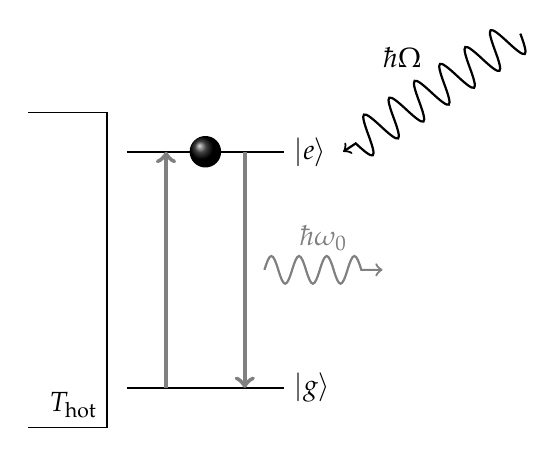
\begin{tikzpicture}[scale = 1]
    % Drawing 2-level system
    \draw[thick] (0,0) -- (2,0) node[right] {$\vert g\rangle$};
    \draw[thick] (0,3) -- (2,3) node[right] {$\vert e\rangle$};
    \draw (-1.25,3.5) -- (-0.25,3.5) -- (-0.25,-0.5) node[above left] {$T_{\mathrm{hot}}$} -- (-1.25,-0.5);
    \draw[gray,->] [ultra thick] (0.5,0) -- (0.5,3);
    \draw[gray,->] [ultra thick] (1.5,3) -- (1.5,0);
    \draw[
      gray,thick,->,
      snake=coil,
      segment aspect=0,
      segment amplitude=5pt,
      segment length=10pt
    ]  (1.75,1.5) -- (3.25,1.5);
    \draw[
      thick,->,
      snake=coil,
      segment aspect=0,
      segment amplitude=7pt,
      segment length=11pt
    ]  (5,4.5) -- (2.75,3);
    \shade[ball color=black] (1,3) circle (0.2);
    % Labelling 2-level system
    \node at (2.5,1.9) [gray] {$\hbar \omega_0$};
    \node at (3.5,4.2) {$\hbar \Omega$};
  \end{tikzpicture}
}

\begin{document}

% This is a sample titlepage design
\makethesistitle

\declaration

\tableofcontents

\chapter{Introduction}
\epigraph{The bomb has been planted!}{Counter Terrorist (1999--present)}	

Welcome to the \thesis\ layout. This layout is based on Nicolai Lang's thesis template, but with my improvements. In the following text I will describe, what this package offers.

\section{Options}

You can load the package with a few options.
\begin{verbatim}
\usepackage[<options>]{thesis}
\end{verbatim}
The several choices for \verb|<options>| are:
\begin{itemize}
\item \verb|nouglyheaders|: This will disable the headers used by Nicolai Lang in his thesis. I don't consider the scaled chapter number and the dotted line good style.
\item \verb|noweirdcolors|: In the original layout the background color of each theorem box was defined in terms of the header color. It is better style to use the same background color everywhere. You can get a consistent background color (\texttt{gray0}) with this option.
\item \verb|dottedsubsection|: In the thesis, the subsections don't have a dotted line beneath their title. If you want one, use this option.
\item \verb|nostyledepigraph|: The styling of the epigraph can be turned of by this option.
\item \verb|nowrongspacing|: Originally in the environment \verb|markforumula| you have to much space on the right, such that the equation number got displaced. This option cancels this extra space.
\item \verb|consistency|: This combines the options \verb|nouglyheaders|, \verb|noweirdcolors| and \verb|nowrongspacing| to give you a more consistent layout. This manual is typeset with this option.
\item \verb|styledtoc|: Typesets the Table of Contents in a style manner (no enddot for numbers, coloured chapters, left aligned page numbers. This manual is typeset with this option.
\item \verb|alignedtoc|: The Table of Contents is left aligned (no indentation for lower sectioning levels. This has no effect without \verb|styledtoc|.
\item \verb|dottedtoc|: Numbers in the Table of Contents are right aligned with dot leaders. This has no effect without \verb|styledtoc|.
\item \verb|notitles|: Turns off styling of chapters, sections, etc.
\end{itemize}

Furthermore this package offers some new commands.

It is a pain to handle unnumbered sections with \verb|titlesec| and the solutions are all very buggy. That's why \thesis\ offers you \verb|numfix{<section>}|. You use it like
\begin{verbatim}
\numfix{\section*{Options}}
\end{verbatim}
Then you will get the dotted line under the section commands right.

Also there is \verb|\makethesistitle|. It typesets a titlepage similar to \verb|\maketitle|, but with some extra stuff. For it to work you will need the following statements before issuing \verb|\makethesistitle|:
\begin{verbatim}
\title{<title>}
\author{<list of authors>} % don't use \and
\university{<university>}
\institute{<institute>}
\supervisor[<Supervised by>]{<supervisor of the thesis>}
\thesisname{<default: Thesis>} % optional
\secondarycorrector[<Secondary corrector>]{<other supervisor>} % optional
\date{<date>} % optional
\end{verbatim}

With the command \verb|\declaration| you get a page which holds a statutory declaration, that you did the work yourself (The starred version \verb|\declaration*| does no \verb|\cleardoublepage| before and doesn't set the pagestyle to  \verb|empty|). If you don't like the title or the body text, you can customize these be doing \verb|\renewcommand| on two items \verb|\declarationtitle| and \verb|\declarationbody|. Seperate lines by \verb|\\|.
\begin{verbatim}
\renewcommand\declarationtitle{Statutory Declaration}
\renewcommand\declarationbody{
  I herewith formally declare that I have written the submitted
  thesis independently. I did not use any outside support except
  for the quoted literature and other sources mentioned in the paper.\\
  I clearly marked and separately listed all of the literature
  and all of the other sources which I employed when producing
  this academic work, either literally or in content.
}
\end{verbatim}

\section{Customizing the headings}

You can control the sizes of the boxes, which hold the sectioning numbers via macros like \verb|\chapterboxwidth|. In the following you can see the available lengths and their default values:
\begin{verbatim}
\chapterboxwidth=8em
\chapterboxheight=20ex
\sectionboxwidth=2.3em
\sectionboxheight=3.5ex
\subsectionboxwidth=2.6em
\subsectionboxheight=3ex
\subsubsectionboxwidth=3em
\subsubsectionboxheight=2ex
\end{verbatim}
This manual sets
\begin{verbatim}
\chapterboxheight=15ex
\chapterboxwidth=10em
\end{verbatim}
Keep in mind, that you will need to set this \emph{after} you loaded \thesis.

\section{Using the Layout with article-like Classes}

The package automatically checks, if \verb|\chapter| is defined and provides a style suited for articles, if \verb|\chapter| isn't defined.

\section{Packages loaded by \thesis}

The following packages are loaded by \thesis\ with the listed options. If you want to specify any extra options to these packages, do so via
\begin{verbatim}
\PassOptionsToPackage{<options>}{<package>}
\end{verbatim}
before \verb|\usepackage{thesis}|.

\subsection{List of loaded packages}

\begin{verbatim}
amssymb
xcolor
mdframed   -   framemethod=tikz
fancyhdr
caption
titlesec   -   explicit
tocloft    -   titles
tikz
epigraph
csquotes
\end{verbatim}

\begin{itemize}
  \item \verb|csquotes| will not be loaded if option \verb|nostyledepigraph| is employed.
  \item \verb|tocloft| will only be loaded if option \verb|styledtoc| is active.
  \item \verb|titlesec| will not be loaded if \verb|notitles| is specified.
\end{itemize}


\chapter{Definitions}
\epigraph{I'll be back!}{Arnold Schwarzenegger \cite{abc}}

\section{Colors}

The colors available by default from the layout are listed in table~\ref{tab:colors}.

There are some aliases for colors, for instance
\begin{itemize}
\item \verb|\definecolor{captioncolor}{named}{parablue}|
\end{itemize}

You redirect these easily by doing things like
\begin{verbatim}
\definecolor{captioncolor}{named}{tikzorange}
\end{verbatim}

\begin{table}[ht]
  \centering\ttfamily
  \begin{tabular}{ccc}
    \toprule
    {\normalfont Color} & {\normalfont Type} & {\normalfont Code} \\
    \midrule
    \rowcolor{intlink}    {intlink} & {HTML} & {424B5C} \\
    \rowcolor{top}        {top} & {HTML} & {646974} \\
    \rowcolor{codeback}   {codeback} & {HTML} & {F2F2F2} \\
    \rowcolor{seccolor}   {seccolor} & {HTML} & {646974} \\
    \rowcolor{secblock}   {secblock} & {HTML} & {2C3038} \\
    \rowcolor{parablue}   {parablue} & {HTML} & {1357BD} \\
    \rowcolor{myblue}     {myblue} & {HTML} & {1357BD} \\
    \rowcolor{refblue}    {refblue} & {HTML} & {26B1FF} \\
    \rowcolor{mygreen}    {mygreen} & {HTML} & {10741E} \\
    \rowcolor{mygray}     {mygray} & {HTML} & {2C3038} \\
    \rowcolor{mylightgray}{mylightgray} & {HTML} & {3661A0} \\
    \rowcolor{dotgray}    {dotgray} & {HTML} & {4B4B52} \\
    \rowcolor{tikzorange} {tikzorange} & {HTML} & {FF8811} \\
    \rowcolor{tikzgrey}   {tikzgrey} & {HTML} & {686868} \\
    \rowcolor{tikzlight}  {tikzlight} & {HTML} & {DEE0E0} \\
    \rowcolor{tikzred}    {tikzred} & {HTML} & {E58A19} \\
    \rowcolor{tikzgreen}  {tikzgreen} & {HTML} & {2E7CBF} \\
    \rowcolor{gray0}      {gray0} & {HTML} & {F1F1F1} \\
    \rowcolor{gray1}      {gray1} & {HTML} & {DFDFDF} \\
    \rowcolor{gray2}      {gray2} & {HTML} & {CDCDCD} \\
    \rowcolor{gray3}      {gray3} & {HTML} & {BBBBBB} \\
    \rowcolor{gray4}      {gray4} & {HTML} & {A6A6A6} \\
    \rowcolor{gray5}      {gray5} & {HTML} & {8E8E8E} \\
    \rowcolor{gray6}      {gray6} & {HTML} & {D6D6D6} \\
    \rowcolor{gray7}      {gray7} & {HTML} & {404040} \\
    \bottomrule
  \end{tabular}
  \caption{Color table.}
  \label{tab:colors}
\end{table}

\section{Theorems}

Many different styles of theorems are provided by \thesis. In the following you will find a showcase with the name and some sample text. Most of them are equivalent in their style, but the title differs. \emph{Note that these boxes CANNOT BREAK through pages}.
\begin{verbatim}
\begin{<title>}[\texttt{<title>}]
  Sample text.
\end{<title>}
\end{verbatim}

\begin{result}[\texttt{result}]
  Sample text.
\end{result}

\begin{definition}[\texttt{definition}]
  Sample text.
\end{definition}

\begin{proposition}[\texttt{proposition}]
  Sample text.
\end{proposition}

\begin{lemma}[\texttt{lemma}]
  Sample text.
\end{lemma}

\begin{theorem}[\texttt{theorem}]
  Sample text.
\end{theorem}

\begin{corollary}[\texttt{corollary}]
  Sample text.
\end{corollary}

\begin{conjecture}[\texttt{conjecture}]
  Sample text.
\end{conjecture}

\begin{note}[\texttt{note}]
  Sample text.
\end{note}

\subsection{markforumla}

You can highlight a formula by enclosing it in the \verb|markformula| environment.
\begin{verbatim}
\begin{markformula}
  \begin{equation}
    \nabla\cdot\vec{E} = 4 \pi \varrho
  \end{equation}
  \begin{equation}
    \int_{\Omega}\nabla\cdot\vec{E}(\vec{r})\,\mathrm{d}^3r
    = \oint_{\partial\Omega}\vec{E}(\vec{r})\cdot\vec{n}\,\mathrm{d}^2r
  \end{equation}
\end{markformula}
\end{verbatim}
\begin{markformula}
  \begin{equation}
    \nabla\cdot\vec{E} = 4 \pi \varrho
  \end{equation}
  \begin{equation}
    \int_{\Omega}\nabla\cdot\vec{E}(\vec{r})\,\mathrm{d}^3r
    = \oint_{\partial\Omega}\vec{E}(\vec{r})\cdot\vec{n}\,\mathrm{d}^2r
  \end{equation}
\end{markformula}

\section{Captions}

Captions are defined to be centered if the caption is only one line. More lined captions are aligned left, without indentation.

\begin{figure}[htpb]
  \centering
  \includegraphics[width=5cm,height=2cm]{demo}
  \caption{Sample caption, which is so long that it occupies two lines. You can see that the second line has no indentation at all.}
  \label{fig:xyz}
\end{figure}

\section{itemize}

The itemize is customized. In the original thesis, a picture was included for the itemize symbol. I tried to reproduce the picture in Ti\textit{k}Z which is now the default itemize symbol. \labelitemi

\section{epigraph}

You can start off every chapter with an inspirational quote, like in this manual. You use it like
\begin{verbatim}
\epigraph{<quote>}{<author>}
\end{verbatim}

% Some sample text
\appendix
\blinddocument

\pagestyle{references}
\begin{thebibliography}{99}
\bibitem{abc}
Arnold Schwarzenegger.
\newblock {\em Terminator 2}.
\newblock Universal Studios, 2012.

\bibitem{knuth:ct:e}
Donald~E. Knuth.
\newblock {\em Computer Modern Typefaces}, volume~E.
\newblock Addison-Wesley.

\bibitem{knuth:ct}
Donald~E. Knuth.
\newblock {\em Computers \& Typesetting}.
\newblock Addison-Wesley.

\bibitem{knuth:ct:related}
Donald~E. Knuth.
\newblock {\em Computers \& Typesetting}.
\newblock Addison-Wesley.

\bibitem{knuth:ct:d}
Donald~E. Knuth.
\newblock {\em METAFONT: The Program}, volume~D.
\newblock Addison-Wesley.

\bibitem{knuth:ct:c}
Donald~E. Knuth.
\newblock {\em The METAFONTbook}, volume~C.
\newblock Addison-Wesley.

\bibitem{knuth:ct:a}
Donald~E. Knuth.
\newblock {\em The \TeX book}, volume~A.
\newblock Addison-Wesley.

\bibitem{knuth:ct:b}
Donald~E. Knuth.
\newblock {\em \TeX: The Program}, volume~B.
\newblock Addison-Wesley.

\bibitem{moraux}
Paul Moraux.
\newblock Le \emph{De Anima} dans la tradition gr{\`e}cque.
\newblock In G.~E.~R. Lloyd and G.~E.~L. Owen, editors, {\em Aristotle on Mind
  and the Senses}, pages 281--324. Cambridge University Press.

\bibitem{nietzsche:ksa1}
Friedrich Nietzsche.
\newblock {\em Die Geburt der Trag{\"o}die. Unzeitgem{\"a}{\ss}e Betrachtungen
  I--IV. Nachgelassene Schriften 1870--1973}, volume~1.
\newblock Deutscher Taschenbuch-Verlag and Walter de Gruyter, 2 edition.

\bibitem{nietzsche:ksa}
Friedrich Nietzsche.
\newblock {\em S{\"a}mtliche Werke}.
\newblock Deutscher Taschenbuch-Verlag and Walter de Gruyter, 2 edition.

\bibitem{nietzsche:historie}
Friedrich Nietzsche.
\newblock {\em Unzeitgem{\"a}sse Betrachtungen. Zweites St{\"u}ck}, volume~1,
  pages 243--334.
\newblock Deutscher Taschenbuch-Verlag and Walter de Gruyter.

\bibitem{nussbaum}
Martha Nussbaum.
\newblock {\em Aristotle's ``De Motu Animalium''}.
\newblock Princeton University Press.

\bibitem{vangennep:trans}
Arnold van Gennep.
\newblock {\em The Rites of Passage}.
\newblock University of Chicago Press, 1960.

\bibitem{vazques-de-parga}
Luis V{\'a}zques{ de }Parga, Jos{\'e}~Mar{\'i}a Lacarra, and Juan
  Ur{\'i}a~R{\'i}u.
\newblock {\em Las Peregrinaciones a Santiago de Compostela}.
\newblock Iberdrola.
\newblock Ed. facs. de la realizada en 1948--49.

\bibitem{brandt}
Ahasver von Brandt and Erich Hoffmann.
\newblock Die nordischen l{\"a}nder von der mitte des 11.~jahrhunderts bis
  1448.
\newblock In Ferdinand Seibt, editor, {\em Europa im Hoch- und
  Sp{\"a}tmittelalter}, number~2 in Handbuch der europ{\"a}ischen Geschichte,
  pages 884--917. Klett-Cotta.

\bibitem{wassenberg}
Jan Wassenberg and Peter Sanders.
\newblock Faster radix sort via virtual memory and write-combining.

\bibitem{weinberg}
Steven Weinberg.
\newblock A model of leptons.
\newblock 19:1264--1266.

\bibitem{westfahl:space}
Gary Westfahl.
\newblock The true frontier.
\newblock In {\em Space and Beyond\/} \cite{westfahl:frontier}, pages 55--65.
\end{thebibliography}

\end{document}
